\documentclass[aspectratio=169]{beamer}

\usetheme{Boadilla}
\usefonttheme{professionalfonts}
\setbeamertemplate{navigation symbols}{}
\setbeamertemplate{itemize items}[circle]
\setbeamertemplate{enumerate items}[default]
\setbeamertemplate{headline}{}

\usepackage[utf8]{inputenc}
\usepackage[T1]{fontenc}
\usepackage{lmodern}
\usepackage{amsmath}
\usepackage{booktabs}
\usepackage{tabularx}
\usepackage{array}
\usepackage{hyperref}
\usepackage[strings]{underscore}
\usepackage{listings}
\usepackage{tikz}
\usetikzlibrary{arrows.meta,positioning,fit,calc,shapes.geometric}
\usepackage{xcolor}

\definecolor{courseblue}{HTML}{12355B}
\definecolor{coursegold}{HTML}{C98A2E}
\definecolor{courseice}{HTML}{EEF3F8}
\definecolor{coursegreen}{HTML}{2F6B4F}
\definecolor{coursegray}{HTML}{4B5563}
\definecolor{codebg}{HTML}{F7F9FC}
\definecolor{codecomment}{HTML}{5E6C84}
\definecolor{codestring}{HTML}{0B6E4F}

\setbeamercolor{palette primary}{bg=courseblue,fg=white}
\setbeamercolor{palette secondary}{bg=coursegold,fg=white}
\setbeamercolor{palette tertiary}{bg=courseblue,fg=white}
\setbeamercolor{palette quaternary}{bg=coursegold,fg=white}
\setbeamercolor{structure}{fg=courseblue}
\setbeamercolor{frametitle}{bg=courseice,fg=courseblue}
\setbeamercolor{title}{fg=courseblue}
\setbeamercolor{block title}{bg=courseblue,fg=white}
\setbeamercolor{block body}{bg=courseice,fg=black}
\setbeamercolor{normal text}{fg=black,bg=white}
\setbeamercolor{alerted text}{fg=coursegold}

\setbeamerfont{footline}{size=\scriptsize}

\setbeamertemplate{footline}{
  \leavevmode
  \hbox{
    \begin{beamercolorbox}[wd=.33\paperwidth,ht=2.8ex,dp=1.2ex,leftskip=0.8em]{palette primary}%
      University of Trieste
    \end{beamercolorbox}%
    \begin{beamercolorbox}[wd=.49\paperwidth,ht=2.8ex,dp=1.2ex,center]{palette tertiary}%
      \coursename{} \textbar{} \coursecode
    \end{beamercolorbox}%
    \begin{beamercolorbox}[wd=.18\paperwidth,ht=2.8ex,dp=1.2ex,rightskip=0.8em plus1fil]{palette secondary}%
      \insertframenumber{} / \inserttotalframenumber
    \end{beamercolorbox}%
  }
}

\hypersetup{
  colorlinks=true,
  linkcolor=courseblue,
  urlcolor=coursegreen
}

\lstdefinestyle{coursepython}{
  language=Python,
  basicstyle=\ttfamily\footnotesize,
  keywordstyle=\color{courseblue}\bfseries,
  commentstyle=\color{codecomment}\itshape,
  stringstyle=\color{codestring},
  showstringspaces=false,
  columns=fullflexible,
  keepspaces=true,
  frame=single,
  framerule=0.6pt,
  rulecolor=\color{courseblue},
  backgroundcolor=\color{codebg},
  xleftmargin=0.4em,
  xrightmargin=0.4em,
  aboveskip=0.4em,
  belowskip=0.2em
}

\newcommand{\coursename}{Data-driven Systems Engineering}
\newcommand{\coursecode}{440MI / 305SM}
\newcommand{\coursefooter}{}

\newcommand{\learninggoals}[1]{
  \begin{block}{Learning goals}
  #1
  \end{block}
}

\newcommand{\repoactivity}[1]{
  \begin{block}{Repo activity}
  #1
  \end{block}
}

\newcommand{\readinglist}[1]{
  \begin{block}{Papers and materials}
  {\footnotesize #1}
  \end{block}
}

\newcommand{\coursecontextframe}[5]{
  \begin{frame}{Course Map and Running Cases}
  \centering
  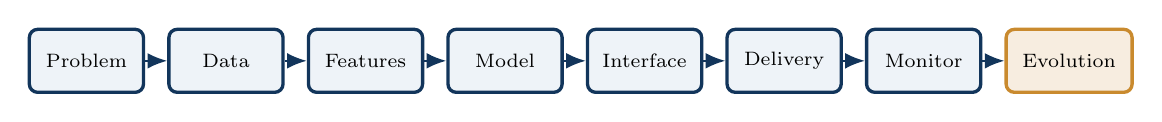
\begin{tikzpicture}[node distance=0.28cm]
  \node[flowbox, minimum width=1.45cm, minimum height=0.8cm] (problem) {\scriptsize Problem};
  \node[flowbox, minimum width=1.45cm, minimum height=0.8cm, right=of problem] (data) {\scriptsize Data};
  \node[flowbox, minimum width=1.45cm, minimum height=0.8cm, right=of data] (features) {\scriptsize Features};
  \node[flowbox, minimum width=1.45cm, minimum height=0.8cm, right=of features] (model) {\scriptsize Model};
  \node[flowbox, minimum width=1.45cm, minimum height=0.8cm, right=of model] (interface) {\scriptsize Interface};
  \node[flowbox, minimum width=1.45cm, minimum height=0.8cm, right=of interface] (delivery) {\scriptsize Delivery};
  \node[flowbox, minimum width=1.45cm, minimum height=0.8cm, right=of delivery] (monitor) {\scriptsize Monitor};
  \node[accentbox, minimum width=1.6cm, minimum height=0.8cm, right=of monitor] (evolution) {\scriptsize Evolution};
  \foreach \a/\b in {problem/data,data/features,features/model,model/interface,interface/delivery,delivery/monitor,monitor/evolution} {
    \draw[arrow] (\a) -- (\b);
  }
  \end{tikzpicture}

  \vspace{0.5em}
  \begin{block}{Today in the course}
  \textbf{Focus:} #1

  \textbf{Bridge:} #2
  \end{block}

  \begin{columns}[T]
  \column{0.48\textwidth}
  \begin{block}{Fraud case}
  {\footnotesize #3}
  \end{block}
  \column{0.48\textwidth}
  \begin{block}{Pasteurization case}
  {\footnotesize #4}
  \end{block}
  \end{columns}

  \vspace{0.3em}
  {\footnotesize \textbf{Course thread:} #5}
  \coursefooter
  \end{frame}
}

\newcommand{\classclosingframe}[4]{
  \begin{frame}{From This Class to the Next}
  \begin{block}{What stays with us}
  #1
  \end{block}

  \begin{columns}[T]
  \column{0.48\textwidth}
  \begin{block}{Project use}
  {\footnotesize #2}
  \end{block}
  \column{0.48\textwidth}
  \begin{block}{Next connection}
  {\footnotesize #3}
  \end{block}
  \end{columns}

  \vspace{0.3em}
  {\footnotesize \textbf{Course thread:} #4}
  \coursefooter
  \end{frame}
}

\tikzset{
  flowbox/.style={
    rounded corners=3pt,
    draw=courseblue,
    fill=courseice,
    very thick,
    minimum width=2.2cm,
    minimum height=0.9cm,
    align=center,
    font=\small
  },
  accentbox/.style={
    rounded corners=3pt,
    draw=coursegold,
    fill=coursegold!15,
    very thick,
    minimum width=2.2cm,
    minimum height=0.9cm,
    align=center,
    font=\small
  },
  arrow/.style={
    -{Latex[length=2.5mm,width=2mm]},
    thick,
    draw=courseblue
  }
}


\title{Class 5: Modeling, Evaluation, and Adaptation}
\author{\coursename}
\date{}

\begin{document}

\frame{\titlepage \coursefooter}

\begin{frame}{Agenda}
\begin{itemize}
\item Modeling as abstraction and representation choice.
\item Matching model families to problem types and constraints.
\item Evaluation beyond accuracy.
\item Offline learning, online learning, and adaptation.
\item How modeling choices affect deployment and monitoring later.
\end{itemize}
\coursefooter
\end{frame}

\begin{frame}{Learning goals}
\learninggoals{
\begin{itemize}
\item Frame modeling as an engineering choice rather than a leaderboard game.
\item Match model types to data, objectives, and operational constraints.
\item Evaluate models using metrics that reflect the real task.
\item Explain when adaptation or online learning becomes necessary.
\end{itemize}
}
\coursefooter
\end{frame}

\coursecontextframe
{Model choice, evaluation, and adaptation.}
{This class turns engineered features into predictive behavior and prepares the later discussion on serving, deployment, and monitoring.}
{In the fraud case, the key question is how to score rare events with metrics and thresholds that reflect business cost.}
{In the pasteurization case, the key question is whether forecasting or state-aware prediction helps operators anticipate abnormal behavior.}
{The course thread now shifts from representation quality to decision quality and operational trade-offs.}

\begin{frame}{What is modeling?}
\begin{itemize}
\item Modeling is the process of representing patterns in data so the system can generalize to unseen cases.
\item Every model encodes assumptions about structure, noise, and decision boundaries.
\item Choosing a model means choosing a trade-off among accuracy, interpretability, speed, and maintainability.
\end{itemize}
\coursefooter
\end{frame}

\begin{frame}{Useful modeling questions}
\begin{enumerate}
\item What decision or prediction are we supporting?
\item What kind of target do we have: class, score, or continuous value?
\item What kinds of errors are expensive?
\item How fast must training and inference be?
\item How often do we expect the data distribution to change?
\end{enumerate}
\coursefooter
\end{frame}

\begin{frame}{Model families in context}
\begin{tabularx}{\textwidth}{>{\bfseries}l X}
Linear models & Fast, simple, and often strong baselines. \\
Tree-based models & Good for heterogeneous tabular data and nonlinearity. \\
Probabilistic models & Useful when uncertainty and conditional structure matter. \\
Neural networks & Powerful for large unstructured or highly nonlinear problems. \\
Online models & Update incrementally as new observations arrive. \\
\end{tabularx}
\coursefooter
\end{frame}

\begin{frame}{More realistic examples}
\begin{itemize}
\item Fraud detection: random forest or gradient boosting with threshold tuning.
\item Streaming weather prediction: online linear regression with River.
\item Pasteurization forecasting: incremental regression plus drift alerts.
\item Industrial anomaly detection: useful only if alert cost and false positives are understood.
\end{itemize}
\coursefooter
\end{frame}

\begin{frame}{Evaluation must match the task}
\begin{itemize}
\item Imbalanced classification needs precision, recall, PR-AUC, and threshold analysis.
\item Regression needs error magnitude metrics such as MAE or RMSE.
\item Calibrated probabilities matter when downstream action depends on confidence.
\item Operational cost matters as much as numerical score.
\end{itemize}
\coursefooter
\end{frame}

\begin{frame}[fragile]{Repository example: fraud model training pipeline}
\begin{lstlisting}[style=coursepython]
X = df.drop("is_fraud", axis=1)
y = df["is_fraud"]

X_train, X_test, y_train, y_test = train_test_split(
    X, y, test_size=0.2, random_state=42, stratify=y
)

scaler = StandardScaler()
X_train_scaled = scaler.fit_transform(X_train)
X_test_scaled = scaler.transform(X_test)
\end{lstlisting}
\begin{itemize}
\item `streamlit/modeling.py` gives a concrete tabular classification flow.
\item Stratification matters because fraud is rare and naive splits can distort the class balance.
\end{itemize}
\coursefooter
\end{frame}

\begin{frame}{Fraud dataset reality: extreme class imbalance}
\centering
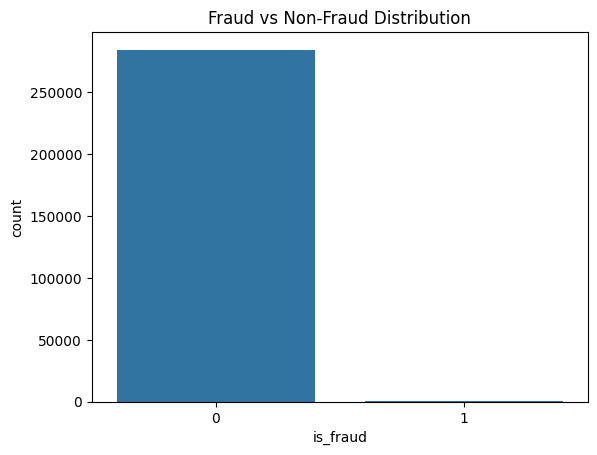
\includegraphics[height=0.72\textheight]{images/class05_fraud_class_balance.png}

{\scriptsize From `Credit_Card_Fraud_Detection_Solution.ipynb`: the first modeling challenge is not algorithm choice but the rarity of the positive class.}
\coursefooter
\end{frame}

\begin{frame}[fragile]{Repository example: fit, predict, and inspect errors}
\begin{lstlisting}[style=coursepython]
cls = RandomForestClassifier(
    n_estimators=200, random_state=42, n_jobs=-1
)
cls.fit(X_train_scaled, y_train)

y_pred = cls.predict(X_test_scaled)
print(confusion_matrix(y_test, y_pred))
print(classification_report(y_test, y_pred, digits=4))
\end{lstlisting}
\begin{itemize}
\item This is a better discussion anchor than accuracy alone because the confusion matrix exposes missed fraud cases directly.
\item The classification report opens the door to threshold and cost-sensitive evaluation.
\end{itemize}
\coursefooter
\end{frame}

\begin{frame}{Model interpretation: top feature importances}
\centering
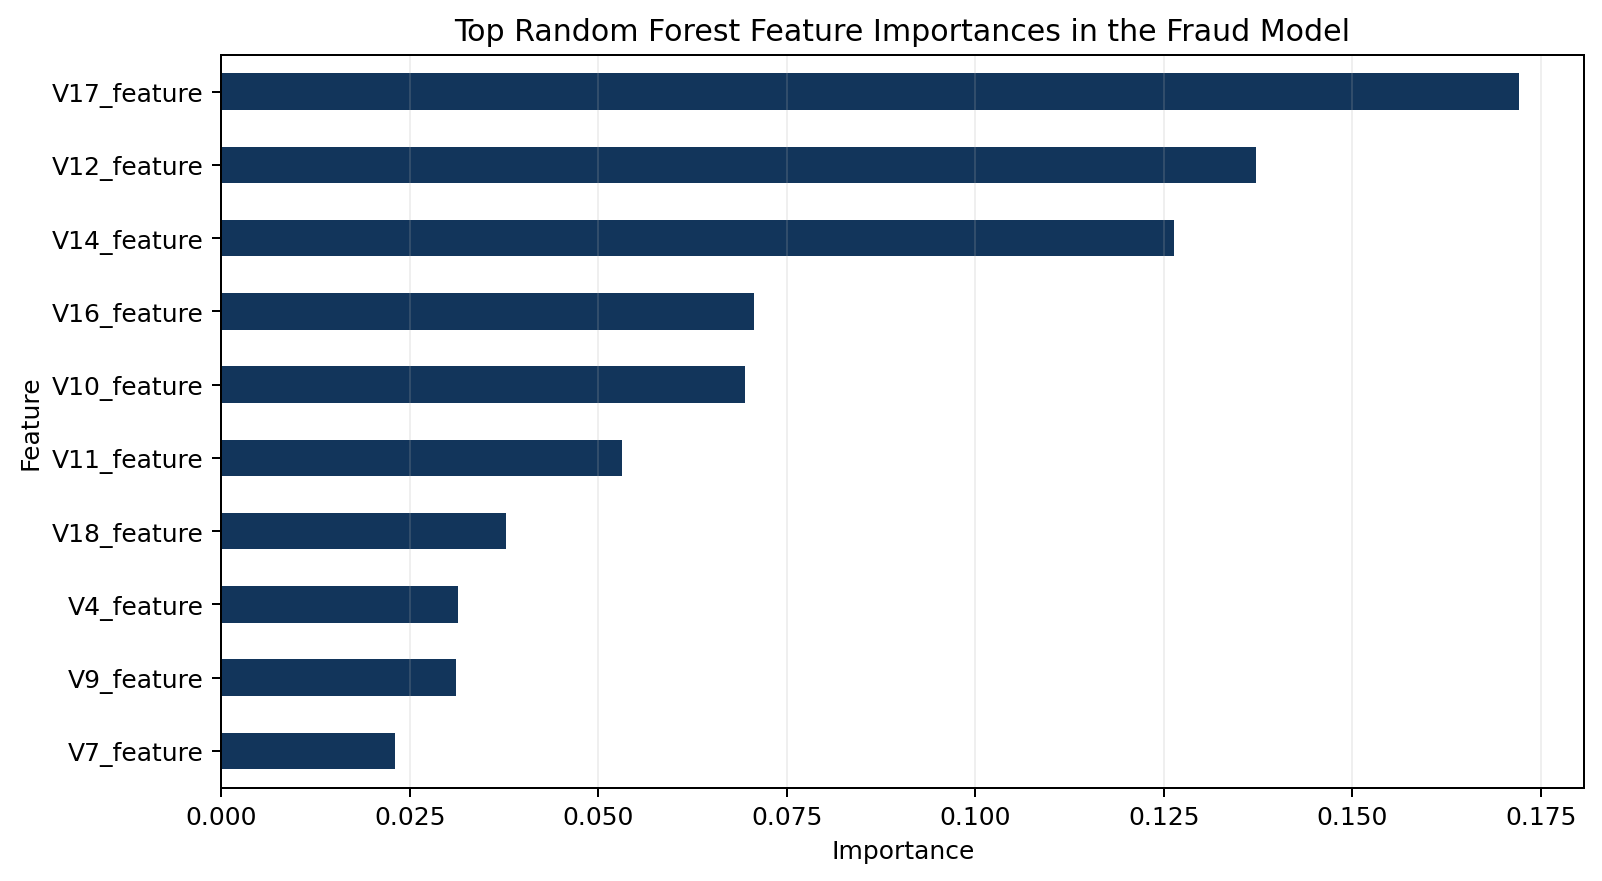
\includegraphics[height=0.72\textheight]{images/class05_feature_importance.png}

{\scriptsize Generated from the saved `streamlit/model.pkl`: tree-based models can highlight influential variables, but importance is still not the same as causality.}
\coursefooter
\end{frame}

\begin{frame}{Why accuracy can fail badly}
\begin{block}{Fraud example}
If only 0.2\% of transactions are fraudulent, a model that predicts ``legitimate'' every time may look highly accurate while being operationally useless.
\end{block}
\begin{itemize}
\item This is why threshold, recall, and precision are part of the engineering conversation.
\end{itemize}
\coursefooter
\end{frame}

\begin{frame}{Distribution shift starts with the raw variables}
\centering
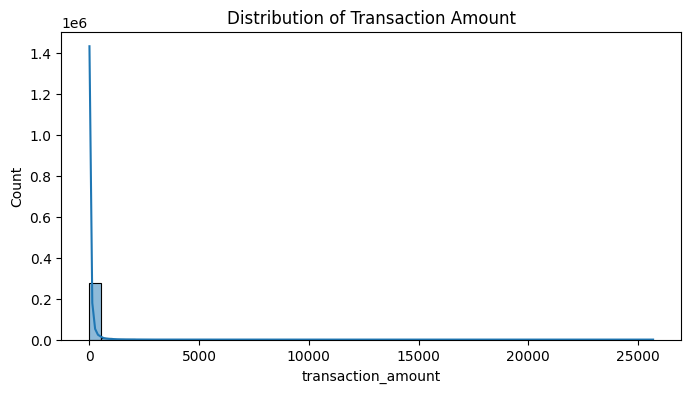
\includegraphics[height=0.72\textheight]{images/class05_transaction_amount_hist.png}

{\scriptsize The transaction amount distribution from the fraud notebook is highly skewed, which is a useful reminder that modeling choices interact with preprocessing and scale.}
\coursefooter
\end{frame}

\begin{frame}{Offline, online, and adaptive learning}
\begin{columns}[T]
\column{0.48\textwidth}
\textbf{Offline}
\begin{itemize}
\item Train on a fixed dataset
\item Easier benchmarking
\item Periodic retraining
\end{itemize}
\column{0.48\textwidth}
\textbf{Online}
\begin{itemize}
\item Update one sample at a time
\item Works on streams
\item Responds faster to change
\end{itemize}
\end{columns}
\vspace{0.6em}
\repoactivity{
`notebooks/Class8_Model_Incremental_learning.ipynb` and `streamlit/pages/App_Stream.py` show how incremental learning changes both evaluation and monitoring.
}
\coursefooter
\end{frame}

\begin{frame}{Why adaptation becomes necessary}
\begin{itemize}
\item User behavior changes.
\item Sensors drift or get recalibrated.
\item Business policies or regulations shift.
\item New classes of errors appear after deployment.
\end{itemize}
\begin{block}{Key point}
Model adaptation is not a sign that the first model failed. It is a recognition that the environment evolves.
\end{block}
\coursefooter
\end{frame}

\begin{frame}[fragile]{Streaming example: incremental learning with River}
\begin{lstlisting}[style=coursepython]
model = (
    preprocessing.StandardScaler()
    | linear_model.LinearRegression(optimizer=optim.SGD(0.01))
)
mae = metrics.MAE()

y_pred = model.predict_one({"wind": wind})
model.learn_one({"wind": wind}, temp)
mae.update(temp, y_pred)
\end{lstlisting}
\begin{itemize}
\item This pattern appears in `streamlit/pages/App_Stream.py`.
\item It makes adaptation tangible: the model learns one observation at a time instead of waiting for a full retraining cycle.
\end{itemize}
\coursefooter
\end{frame}

\begin{frame}{Technology links}
\readinglist{
\href{https://scikit-learn.org/stable/}{scikit-learn documentation};\ 
\href{https://scikit-learn.org/stable/modules/model_evaluation.html}{scikit-learn model evaluation guide};\ 
\href{https://riverml.xyz/latest/}{River documentation};\ 
\href{https://riverml.xyz/latest/api/metrics/}{River metrics API}.
}
\coursefooter
\end{frame}

\classclosingframe
{\begin{itemize}
\item Model selection is always tied to the prediction task, the error costs, and the available data.
\item Metrics are decision tools, not decorative scoreboards.
\item Offline training and online adaptation lead to different operational behaviors.
\end{itemize}}
{This is the point where teams can defend a baseline, compare alternatives, and explain why a chosen model fits the constraints of the fraud or pasteurization setting.}
{Class 6 shows how trained models become usable through APIs, dashboards, and human-facing interfaces.}
{A model becomes valuable only when its outputs can be consumed, inspected, and acted on in a real workflow.}

\begin{frame}{Papers and materials}
\readinglist{
\href{https://link.springer.com/book/10.1007/978-0-387-45528-0}{Bishop, Pattern Recognition and Machine Learning};\ 
\href{https://www.cs.cmu.edu/~tom/mlbook.html}{Mitchell, Machine Learning};\ 
\href{https://arxiv.org/abs/2007.06299}{Gama et al., A survey on concept drift adaptation};\ 
\href{https://dl.acm.org/doi/10.1145/2347736.2347755}{Domingos (2012), A Few Useful Things to Know About Machine Learning}.
}
\coursefooter
\end{frame}

\end{document}
